\documentclass[]{standalone}

\usepackage{scalefnt}
\usepackage{tikz}  
\usepackage{tikz-3dplot} 
\usepackage{amssymb,amsfonts,amsmath}
\usepackage{tikz,tkz-euclide}
\usetikzlibrary{arrows,calc,patterns}


\begin{document}
\scalefont{0.5}
    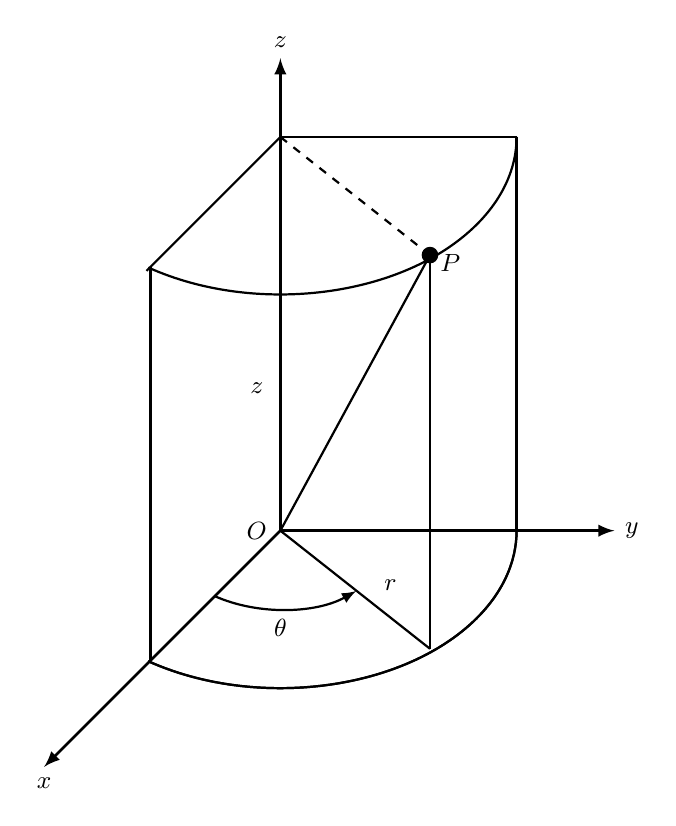
\begin{tikzpicture}[]
    \tikzstyle{every node}=[font=\small]
      \coordinate (O)  at (0,0);
      \coordinate (Ox) at (-3,-3);
      \coordinate (Oy) at (4.243,0);  % sqrt{18}
      \coordinate (Oz) at (0, 6);

      % draw axis 
      \draw[-latex, line width=1] (O)-- (Ox) node[below] {$x$};
      \draw[-latex, line width=1] (O)-- (Oy) node[right] {$y$};
      \draw[-latex, line width=1] (O)-- (Oz) node[above] {$z$};


      % draw arcs
       \draw[thick] ($(0, 0) + (236:3cm and 2cm)$(P) arc
         (236:360:3cm and 2cm);
       \draw[thick] ($(0, 0) + (236:3cm and 2cm)$(P) arc
         (236:360:3cm and 2cm);

       \draw[thick] ($(0, 5) + (236:3cm and 2cm)$(P) arc
         (236:360:3cm and 2cm);

       \draw[thick, -latex] ($(0, 0) + (236:1.5cm and 1cm)$(P) arc
         (236:310:1.5cm and 1cm);

         \coordinate (Phi) at (0,-1) ;
         \node[below] at (Phi) {$\theta$};

    	 \coordinate (Rad) at (1.4,-0.5) ;
         \node[below] at (Rad) {$r$};
         \node[below] at (-0.3,2) {$z$};

      \coordinate (A1) at (0, 5);
      \coordinate (B) at (3, 5);
      \coordinate (C) at (-1.7, 3.3);
      \draw[thick] (A1)--(B);
      \draw[thick] (A1)--(C);

      % radius
      \coordinate (D) at (1.9,-1.5);
      \coordinate (P) at (1.9,3.5);

      \node[] at (-0.3,0) {$O$};
      \draw[thick] (O)--(D);
      \draw[thick] (O)--(P);
      \draw[thick, dashed] (A1)--(P) node[right, yshift=-1mm] {$P$};
      \draw[thick] (D)--(P);
      \fill[black] (P) circle (3pt);

      %\coordinate (A) at (2.6, 4.0);
      %\draw[thick, dashed] (A1)--(A) node[right, yshift=-1mm, xshift=-1mm] {$A$};

      \coordinate (D) at (1.52, 4.42);
      % \fill[black] (D) circle (3pt);


      % verticals on the planes
      \coordinate (H) at (-1.65,-1.65);
      %\fill[black] (H) circle (3pt);
      %
      \coordinate (I) at (-1.65,3.35);
      %\fill[black] (I) circle (3pt);
      \draw[thick] (H) --(I);

      \coordinate (J) at (3,0);
      %\fill[black] (J) circle (3pt);
      \coordinate (K) at (3,5);
      %\fill[black] (K) circle (3pt);
      \draw[thick] (J) --(K);

    \end{tikzpicture}

\end{document}